% --- Program Section ---

\newprogram{Program 9}{Implement knapsack-01(weights: List[int], values: List[int], capacity: int) -> int
utilizing 2D/1D DP methods that accept item properties and return maximum value.}

\subsection*{Code}


\begin{lstlisting}[language=python]
from typing import List


# -------------------------
# 2D Dynamic Programming
# -------------------------
def knapsack_01_2d(
    weights: List[int],
    values: List[int],
    capacity: int
) -> int:

    n = len(weights)

    # dp[i][w] = maximum value using first i items
    # with capacity w
    dp = [[0] * (capacity + 1) for _ in range(n + 1)]

    for i in range(1, n + 1):
        weight = weights[i - 1]
        value = values[i - 1]

        for w in range(capacity + 1):

            # Don't take the item
            dp[i][w] = dp[i - 1][w]

            # Take the item if it fits
            if weight <= w:
                dp[i][w] = max(
                    dp[i][w],
                    value + dp[i - 1][w - weight]
                )

    return dp[n][capacity]

# -------------------------
# 1D Dynamic Programming
# -------------------------
def knapsack_01(
    weights: List[int],
    values: List[int],
    capacity: int
) -> int:

    dp = [0] * (capacity + 1)

    for i in range(len(weights)):
        weight = weights[i]
        value = values[i]

        # Traverse backwards so each item is used only once
        for w in range(capacity, weight - 1, -1):
            dp[w] = max(
                dp[w],
                value + dp[w - weight]
            )

    return dp[capacity]

# -------------------------
# Example
# -------------------------

weights = [1, 3, 4, 5]
values = [1, 4, 5, 7]
capacity = 7

print("2D DP:", knapsack_01_2d(weights, values, capacity))
print("1D DP:", knapsack_01(weights, values, capacity))

\end{lstlisting}

\subsection*{Output}
\begin{center}
    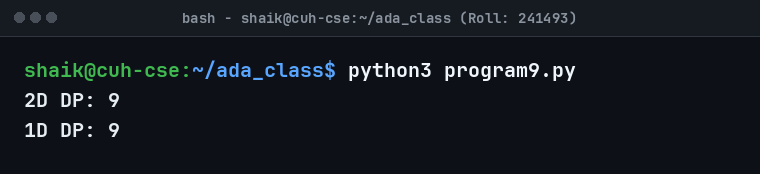
\includegraphics[width=0.88\textwidth]{Images/output_screenshot9.png}
\end{center}

\subsection*{GitHub Scan Code}
\begin{center}
    \begin{minipage}{0.3\textwidth}
        \centering
        % Generates a 2.5cm high QR code directly linking to the code file
        \qrcode[height=3.5cm]{https://github.com/gytdrop/ada_class/blob/main/program9.py} \\[0.2cm]
        \scriptsize\ttfamily Scan to view source code 
    \end{minipage}
\end{center}


% Add a horizontal line that indicates the END of the program.
\vspace{1cm}
\begin{center}
    \rule{1\textwidth}{1pt} % Clean, centered 1pt thick horizontal line
\end{center}